\documentclass[sn-mathphys-num]{sn-jnl}

\usepackage{graphicx}
\usepackage{amsmath}
\usepackage{amssymb}
\usepackage{booktabs}

\begin{document}

\title{Reference Anchoring for Noise-Space Policy Fine-Tuning}

\author[1]{\fnm{} \sur{}}
\affil[1]{\orgdiv{}, \orgname{}, \city{}, \country{}}

\abstract{
Reinforcement learning applied to the latent noise input of a frozen generative
policy raises reward without touching the policy's weights, but it also changes
which of several valid behaviours that policy produces. Methods that aim to keep
this behavioural repertoire regularise the distribution over behavioural modes,
and almost all of them maximise its entropy or a mutual information bound. We
show that this choice makes an unstated assumption. For a reference distribution
that is uniform over $K$ modes, the Kullback-Leibler divergence to that reference
equals $\ln K$ minus the entropy, so anchoring a policy to its pretrained
behaviour and maximising behavioural entropy are the same objective, and no
benchmark whose pretrained policy is uniform can tell them apart. Behaviour
cloning does not produce uniform policies, which is why the distinction matters
in practice and why it has gone unmeasured. We introduce a reference anchor that
penalises total variation between the fine-tuned policy's mode histogram and the
frozen policy's own, has no learned components, and adds one scalar weight to
the objective. Across two manipulation tasks from a diverse-behaviour benchmark,
twenty independently trained backbones and more than one thousand runs, the
anchor holds the fine-tuned policy closer to its pretrained behaviour than
entropy maximisation at every level of reference skew we measured, with a pooled
effect size of 0.91 and 1.14 standard deviations on the two tasks, It reaches this
fidelity without any learned component, where a mutual information method of
comparable fidelity requires both a discriminator and a latent skill space, and
it costs no task success.
}

\keywords{reinforcement learning, generative policies, behavioural diversity,
diffusion models, robot manipulation}

\maketitle

\section{Introduction}\label{sec:intro}

A generative policy trained by behaviour cloning on human demonstrations often
represents several ways of doing the same task. A manipulator that must reach
past an obstacle can pass it on either side; one that must deliver two blocks to
two targets can choose the order. Which of those behaviours the policy produces, and how often, is part of what
the demonstrations taught. That distribution is worth keeping. A policy whose
behaviour distribution matches the one it was cloned from remains predictable to
whoever deployed it, and remains a faithful starting point for any later
adjustment.

Reinforcement learning (RL) can raise the reward of such a policy without
retraining it. Rather than updating the policy's weights, noise-space
methods such as Diffusion Steering Reinforcement Learning (DSRL)
\citep{wagenmaker2025dsrl} freeze the generative policy and train a small
policy over its latent noise input, so the pretrained model is used only as a
decoder. Fine-tuning then requires far less computation and leaves the
pretrained weights intact. It does not, however,
keep behaviour fixed. The noise policy is free to concentrate on whichever region
of the latent space decodes to the highest-reward behaviour, and the behaviour
distribution the demonstrations encoded shifts as a result.

Work that addresses this adds a term rewarding behavioural diversity. Behavioral
Mode Discovery (BMD) \citep{longhini2026bmd} learns a latent skill variable and
maximises a variational lower bound on the mutual information between that
variable and the resulting behaviour, in the manner of unsupervised skill
discovery \citep{eysenbach2018diayn}. Simpler variants maximise the entropy of
the distribution over behavioural modes directly. Both treat diversity as the
quantity to protect.

Fidelity to the pretrained policy is the target we adopt, and it is a different
quantity from diversity. The objectives in current use optimise diversity. Write $C_\phi$ for the distribution over $K$ behavioural modes induced by
the fine-tuned policy, $C_{\mathrm{ref}}$ for the distribution induced by the
frozen policy before fine-tuning, and $u$ for the uniform distribution over the
same $K$ modes. The Kullback-Leibler (KL) divergence of a distribution $p$ from
uniform satisfies
\begin{equation}\label{eq:identity}
  D_{\mathrm{KL}}(p \,\|\, u) \;=\; \ln K - H(p),
\end{equation}
where $H$ denotes Shannon entropy. Minimising the divergence from a uniform
reference and maximising entropy are therefore the same objective. They can only
differ once $C_{\mathrm{ref}}$ itself departs from uniform. A benchmark whose
pretrained policies are near-uniform cannot separate the two, and a method
evaluated only on such a benchmark cannot demonstrate that it preserves anything
in particular.

Pretrained policies are not uniform. Measuring twenty cloned policies over the
six route groups used throughout this paper, their mode distributions lie between
$0.013$ and $1.278$ nats from uniform. Five of those twenty were cloned from an
unmodified demonstration set, and they alone span $0.013$ to $0.395$ nats, so
even balanced demonstrations do not produce a balanced policy. The distinction
that Equation~\ref{eq:identity} removes is therefore present in realistic cases,
and the objective that respects it is not the one in common use.

This paper specifies that objective and measures its effect. Our
contributions are as follows.

First, we identify the reference distribution, not diversity, as the quantity a
mode-preserving regulariser should target, and give the condition
(Equation~\ref{eq:identity}) under which the two are indistinguishable.

Second, we introduce a reference anchor that penalises the total variation
distance between $C_\phi$ and $C_{\mathrm{ref}}$. The anchor has no learned
components, introduces a single scalar weight, and its per-episode coefficient is
bounded by one half regardless of how narrow the pretrained policy's support is.

Third, we evaluate on two manipulation tasks from the Diverse Behaviours
Benchmark for Imitation Learning (D3IL) \citep{jia2024d3il} using behavioural
modes defined by task geometry rather than by clustering. Over twenty
independently trained backbones and more than one thousand fine-tuning runs, the
anchor holds the policy closer to its pretrained behaviour than entropy
maximisation at every measured level of reference skew, and matches a
learned-skill mutual information method at a fraction of its mechanism.

\section{Related Works}\label{sec:related}

\paragraph{Generative policies for manipulation.}
Diffusion models and flow-based models have become a standard policy class for
manipulation. Diffusion Policy \citep{chi2023diffusionpolicy} represents the
action distribution by a denoising process conditioned on observations, which
lets a single policy express several distinct ways of completing a task. Flow
matching \citep{lipman2022flowmatching} and rectified flow
\citep{liu2022rectifiedflow} replace the stochastic denoising chain with a
deterministic transport that is cheaper to integrate, and underpin recent
vision-language-action models such as $\pi_0$ \citep{black2024pi0}. Score-based
policies have also been trained specifically for goal-conditioned manipulation
\citep{reuss2023beso}. Retraining these models requires substantial computation, which motivates
fine-tuning schemes that leave their weights unchanged.

\paragraph{Reinforcement learning in the latent space of a frozen policy.}
DSRL \citep{wagenmaker2025dsrl} formulates fine-tuning as control over the noise
input of a frozen generative policy, training a compact policy over that input
with an off-policy algorithm \citep{haarnoja2018sac}. Because the decoder is
fixed and deterministic for flow-based models, the mapping from noise to action
is differentiable and the search space is small. The resulting policy is still a
reweighting of the pretrained one, which is what makes a fidelity objective
meaningful here and what distinguishes this setting from fine-tuning that updates
the generative weights directly.

\paragraph{Preserving behavioural diversity.}
BMD \citep{longhini2026bmd} conditions the policy on a latent skill index and
trains a discriminator to recover that index from the resulting behaviour, using
the variational mutual information bound as an intrinsic reward. The construction
follows unsupervised skill discovery \citep{eysenbach2018diayn}, where the same
bound is used to learn skills without any task reward. Both discover their own
notion of a mode. A lighter alternative, and the one closest to our setting,
maximises the entropy of a histogram over externally defined modes directly. Our
analysis applies to this family as a whole, since Equation~\ref{eq:identity}
relates any entropy-maximising objective to anchoring against a uniform
reference.

\paragraph{Benchmarks that admit several solutions.}
Measuring mode preservation requires tasks with more than one valid solution.
D3IL \citep{jia2024d3il} was built for this, with tasks whose demonstrations span
a labelled set of behaviours and with the behaviour of a trajectory recoverable
from geometry. Benchmarks assembled for other purposes do not share this
property. LIBERO \citep{liu2023libero}, for instance, is organised around
knowledge transfer, and its tasks largely admit a single solution, which leaves a
mode-preservation term with nothing to act on. We use D3IL for this reason and
define modes by its geometric criteria rather than by clustering actions, so that
the measured quantity does not depend on a learned vocabulary.

\section{Proposed Approach}\label{sec:approach}

\subsection{Problem Formulation}\label{sec:problem}

Let $\pi_\theta$ be a generative policy with parameters $\theta$ fixed throughout.
For a flow-based policy, $\pi_\theta$ maps an observation $o$ and a latent noise
vector $z \in \mathbb{R}^{d}$ to an action $a$. The map integrates a learned
velocity field $v_\theta$ over $M$ Euler steps,
\begin{equation}\label{eq:decode}
  a \;=\; \Phi_\theta(o, z), \qquad
  x_{m+1} \;=\; x_m + \tfrac{1}{M}\, v_\theta\!\left(x_m, \tfrac{m}{M}, o\right),
  \quad x_0 = z,
\end{equation}
so that $\Phi_\theta(o, \cdot)$ is a deterministic and differentiable decoder.
Under the pretrained policy, $z$ is drawn from a standard normal distribution.

Fine-tuning replaces that draw with a learned noise policy $\mu_\phi(z \mid o)$,
a diagonal Gaussian with parameters $\phi$, initialised so that
$\mu_\phi(\cdot \mid o)$ is the standard normal and the composed policy is
therefore identical to $\pi_\theta$ at the start of training. Only $\phi$ is
updated. Writing $\tau$ for a trajectory and $r(\tau)$ for its return, the
unregularised objective is $\mathbb{E}_{\tau \sim \mu_\phi}[r(\tau)]$, which is
the DSRL formulation.

Each trajectory realises one of $K$ behavioural modes. We write $m(\tau) \in
\{1, \dots, K\}$ for the mode of trajectory $\tau$, determined by task geometry
and not by any learned model, and define the mode distribution of a policy as
\begin{equation}\label{eq:cphi}
  C_\phi[k] \;=\; \Pr_{\tau \sim \mu_\phi}\!\left[\, m(\tau) = k \,\right],
  \qquad k = 1, \dots, K .
\end{equation}
The reference distribution $C_{\mathrm{ref}}$ is the same quantity for the frozen
policy, estimated once before fine-tuning by rolling $\pi_\theta$ out under the
standard normal and held fixed thereafter. The problem we address is to raise
$\mathbb{E}[r]$ while keeping $C_\phi$ close to $C_{\mathrm{ref}}$.

\subsection{Reference Versus Entropy}\label{sec:why}

The objectives in common use do not target $C_{\mathrm{ref}}$. They maximise
$H(C_\phi)$, or a variational lower bound on the mutual information between a
latent skill index and the behaviour it produces, which has its optimum at a
uniform distribution over skills. Equation~\ref{eq:identity} shows that when
$C_{\mathrm{ref}} = u$ this coincides exactly with minimising
$D_{\mathrm{KL}}(C_\phi \,\|\, C_{\mathrm{ref}})$. The two objectives are then
the same function of $C_\phi$ up to an additive constant, and any experiment run
on a near-uniform pretrained policy will find them equivalent whatever their
behaviour elsewhere.

Away from that point the objectives have different optima. Entropy
maximisation moves $C_\phi$ toward $u$ from wherever it starts; anchoring moves it
toward $C_{\mathrm{ref}}$. When the pretrained policy favours some behaviours over
others, which Section~\ref{sec:results} shows is the normal case, these are
different destinations, and only the second recovers the behaviour the
demonstrations produced.

\subsection{The Reference Anchor}\label{sec:anchor}

We add to the return a penalty on the distance between the policy's mode
distribution and the reference,
\begin{equation}\label{eq:objective}
  J(\phi) \;=\; \mathbb{E}_{\tau \sim \mu_\phi}\!\left[r(\tau)\right]
  \;-\; \lambda \, D\!\left(C_\phi, C_{\mathrm{ref}}\right),
\end{equation}
with a single scalar weight $\lambda > 0$ controlling the trade-off. For $D$ we
use the total variation distance
\begin{equation}\label{eq:tv}
  D_{\mathrm{TV}}(p, q) \;=\; \tfrac{1}{2} \sum_{k=1}^{K} \left| p[k] - q[k] \right| .
\end{equation}

Total variation is chosen for a property that matters for the estimator below.
The histogram $C_\phi$ is a statistic of the sampled batch, not a differentiable
function of $\phi$. Its gradient therefore comes from the score-function
estimator, which credits each trajectory by the partial derivative of the
penalty at that trajectory's own mode,
\begin{equation}\label{eq:grad}
  \nabla_\phi \, D\!\left(C_\phi, C_{\mathrm{ref}}\right)
  \;=\; \mathbb{E}_{\tau \sim \mu_\phi}\!\left[
    \left. \frac{\partial D}{\partial C_\phi[k]} \right|_{k = m(\tau)}
    \nabla_\phi \log \mu_\phi(\tau)
  \right].
\end{equation}
For total variation that coefficient is
$\tfrac{1}{2}\,\mathrm{sgn}\!\left(C_\phi[k] - C_{\mathrm{ref}}[k]\right)$, whose
magnitude is one half for every mode. The corresponding coefficient for the KL
divergence is $\log\!\left(C_\phi[k] / C_{\mathrm{ref}}[k]\right) + 1$, which
grows without bound as $C_{\mathrm{ref}}[k] \rightarrow 0$. Since a pretrained
policy need not visit every mode, that case arises whenever the reference has
narrow support, and the KL form requires a smoothing parameter to remain usable
where the total variation form does not.

The mode distribution is estimated as an exponential moving average over
iterations rather than from the current batch alone, so that every mode retains a
stable probability even when a batch of sixteen episodes does not visit it. The
penalty coefficient and the reward advantage are each standardised within the
batch before being combined, so that $\lambda$ expresses the relative weight of
the two terms rather than an accident of their units.

The complete method adds one scalar hyperparameter to DSRL, one histogram of
length $K$ held in memory, and one rollout budget spent once before training to
estimate $C_{\mathrm{ref}}$. It introduces no learned components.

\section{Experimental Results}\label{sec:results}

\subsection{Setup}\label{sec:setup}

We evaluate on two manipulation tasks from D3IL \citep{jia2024d3il}. In
\emph{Avoiding}, a manipulator must reach a goal line past three rows of
obstacles, and the behavioural mode is the sequence of sides on which it passes
them, giving $K = 24$ routes that we group into $K = 6$ by the first two rows. In
\emph{Pushing}, two blocks must be delivered to two targets, and the mode is
which block reaches which target in which order, giving $K = 4$. Both modes are
read from object and end-effector geometry using the benchmark's own criteria, so
no clustering step enters the measurement.

The frozen policy for each task is a rectified-flow velocity field
\citep{liu2022rectifiedflow} trained by flow matching on the benchmark's
demonstrations. To vary the reference distribution we reweight the demonstrations
toward a geometric profile over modes before cloning. Behaviour cloning is itself a source of
variation, so we train five backbones per weighting with independent seeds,
giving twenty in total for \emph{Avoiding}. Every result is then indexed by its
own backbone's measured reference skew $D_{\mathrm{TV}}(C_{\mathrm{ref}}, u)$
rather than by the weighting that backbone was trained under.

Reward is given for task success on a subset of modes, so that a return maximiser
has an incentive to narrow its behaviour. Four of the twenty-four routes are
rewarded on \emph{Avoiding} and one of the four on \emph{Pushing}. A run whose
final success rate falls below $0.15$ on \emph{Avoiding} or $0.10$ on
\emph{Pushing} is treated as a failed optimisation and excluded. Because this
threshold conditions on an outcome the treatment affects, Section~\ref{sec:robust}
reports every result both with and without it, and the conclusions drawn below
hold under both. Four objectives are compared, identical in
every respect except the mode term. The first has no mode term and optimises return alone, which is the
unregularised noise-space objective. The
second maximises the entropy of the same geometric mode histogram. The third is
BMD, implemented as a skill-conditioned noise policy together with a
discriminator trained to recover the skill index from the final observation,
using the variational bound as an intrinsic reward. Its skill cardinality is set
to the number of mode groups, and at evaluation its skills are sampled uniformly,
which is the deployment the method is designed for. The fourth is the reference
anchor of Equation~\ref{eq:objective}.

\subsection{Fidelity Measure}

A policy can be close to its reference and close to uniform at once when the two
are themselves close, so a raw distance confounds fidelity with the position of
the reference. We therefore report
\begin{equation}\label{eq:fidelity}
  F(\phi) \;=\; \frac{D_{\mathrm{TV}}(C_\phi, u) - D_{\mathrm{TV}}(C_\phi, C_{\mathrm{ref}})}
                     {D_{\mathrm{TV}}(C_{\mathrm{ref}}, u)} .
\end{equation}
The numerator is positive when the policy is nearer its pretrained behaviour
than uniform and negative when it is nearer uniform. The triangle inequality
bounds it by $\pm D_{\mathrm{TV}}(C_{\mathrm{ref}}, u)$, so the denominator places
every reference on the same scale and $F \in [-1, 1]$. A policy that reproduces
$C_{\mathrm{ref}}$ exactly scores $F = 1$.

\subsection{Main Result}\label{sec:main}

Figure~\ref{fig:main} reports $F$ against measured reference skew for both tasks.
The reference anchor attains the highest fidelity at every one of the eight
levels tested, on two tasks whose behavioural modes are defined by different
physical quantities. Its margin over entropy maximisation widens as the
pretrained policy departs further from uniform. Pooled over levels, the anchor
exceeds entropy maximisation by $0.91$ standard deviations on \emph{Avoiding}
($p < 10^{-4}$) and by $1.14$ on \emph{Pushing} ($p < 10^{-4}$). It exceeds DSRL
by $0.38$ ($p = 0.002$) and $0.71$ ($p = 0.001$), and BMD by $0.31$
($p = 0.009$) and $0.54$ ($p = 0.008$). Table~\ref{tab:main} gives the values.

\begin{figure}[t]
\centering
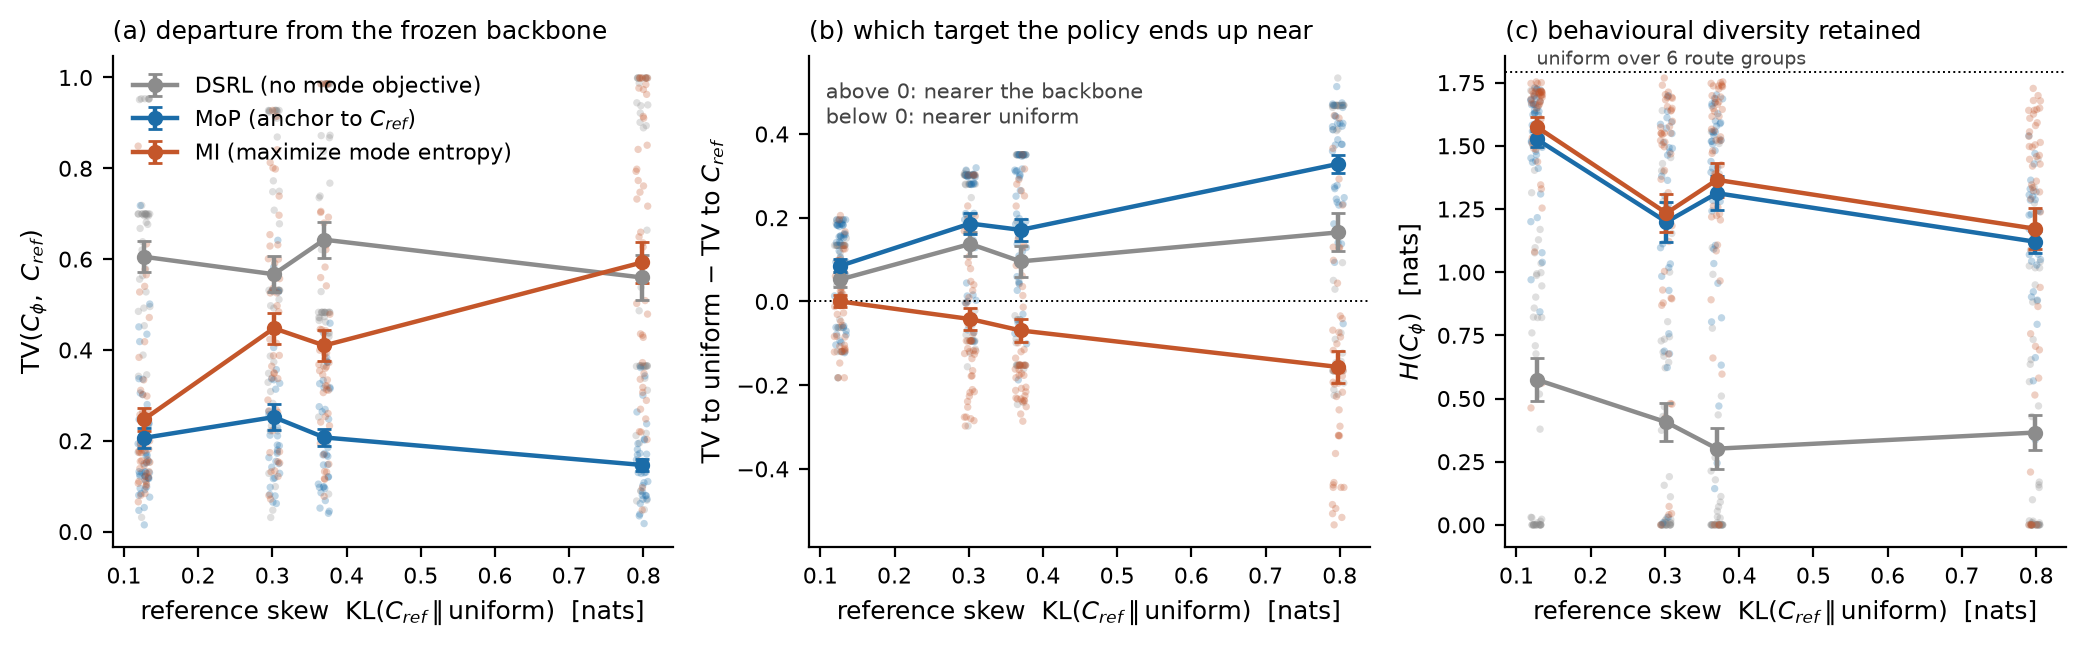
\includegraphics[width=\textwidth]{../figures/fig1_main.png}
\caption{Reference anchoring and the condition that makes it necessary.
(a) The generative policy is frozen and only the noise policy is trained; a
rollout is labelled with its behavioural mode from geometry, and the histogram of
those labels is compared against the frozen policy's own. The four objectives
differ only in the mode term. (b) For a uniform reference, the Kullback-Leibler
divergence from uniform equals $\ln K$ minus the entropy, so the entropy
objective and the anchoring objective trace the same curve and no experiment at
that point can separate them. (c, d) Normalised fidelity $F$ of
Equation~\ref{eq:fidelity} against each backbone's own measured reference skew,
where higher values indicate a fine-tuned policy closer to the behaviour it was
cloned from. Points are means over 6 to 30 runs after the exclusion of
Section~\ref{sec:setup}, and bars are standard errors;
\emph{Avoiding} uses 20 independently trained backbones across four weightings
and \emph{Pushing} uses four. The reference anchor is highest at every level on
both tasks. (e) Effect sizes pooled over levels, with one-sided Welch tests; all
six comparisons favour the anchor, and the comparison against entropy
maximisation is the largest on both tasks.}
\label{fig:main}
\end{figure}

\begin{table}[t]
\caption{Normalised fidelity $F$ by measured reference skew, mean $\pm$ standard
error. Higher is closer to the pretrained policy. The reference anchor is highest
at every level on both tasks.}
\label{tab:main}
\begin{tabular}{@{}llcccc@{}}
\toprule
Task & $D_{\mathrm{TV}}(C_{\mathrm{ref}}, u)$ & No mode term & Mode entropy &
Learned skills & Reference anchor \\
\midrule
Avoiding & 0.24 & $0.188 \pm 0.094$ & $0.210 \pm 0.102$ & $0.155 \pm 0.096$ & $\mathbf{0.367 \pm 0.073}$ \\
Avoiding & 0.33 & $0.425 \pm 0.109$ & $0.270 \pm 0.096$ & $0.517 \pm 0.109$ & $\mathbf{0.621 \pm 0.091}$ \\
Avoiding & 0.46 & $0.629 \pm 0.102$ & $0.155 \pm 0.109$ & $0.567 \pm 0.089$ & $\mathbf{0.735 \pm 0.054}$ \\
Avoiding & 0.55 & $0.556 \pm 0.091$ & $0.156 \pm 0.106$ & $0.714 \pm 0.086$ & $\mathbf{0.813 \pm 0.038}$ \\
\midrule
Pushing & 0.19 & $0.115 \pm 0.178$ & $0.147 \pm 0.134$ & $0.422 \pm 0.147$ & $\mathbf{0.467 \pm 0.186}$ \\
Pushing & 0.36 & $0.417 \pm 0.145$ & $0.014 \pm 0.139$ & $0.371 \pm 0.109$ & $\mathbf{0.647 \pm 0.074}$ \\
Pushing & 0.41 & $0.366 \pm 0.178$ & $0.439 \pm 0.140$ & $0.469 \pm 0.140$ & $\mathbf{0.773 \pm 0.060}$ \\
Pushing & 0.53 & $0.581 \pm 0.142$ & $0.498 \pm 0.147$ & $0.665 \pm 0.114$ & $\mathbf{0.850 \pm 0.057}$ \\
\botrule
\end{tabular}
\end{table}

\subsection{Task Success}

A fidelity objective is only useful if the policy still solves the task.
Table~\ref{tab:success} reports success rates for all four objectives. They are
comparable throughout, so the fidelity reported above is obtained without a
reduction in reward.

\begin{table}[t]
\caption{Task success rate by measured reference skew. The four objectives are
comparable throughout, so the fidelity differences in Table~\ref{tab:main} do not
reflect a trade against task performance.}
\label{tab:success}
\begin{tabular}{@{}llcccc@{}}
\toprule
Task & $D_{\mathrm{TV}}(C_{\mathrm{ref}}, u)$ & No mode term & Mode entropy &
Learned skills & Reference anchor \\
\midrule
Avoiding & 0.24 & 0.632 & 0.670 & 0.665 & 0.626 \\
Avoiding & 0.33 & 0.717 & 0.751 & 0.731 & 0.694 \\
Avoiding & 0.46 & 0.735 & 0.689 & 0.721 & 0.707 \\
Avoiding & 0.55 & 0.722 & 0.617 & 0.767 & 0.688 \\
\midrule
Pushing & 0.19 & 0.256 & 0.269 & 0.292 & 0.254 \\
Pushing & 0.36 & 0.364 & 0.305 & 0.310 & 0.331 \\
Pushing & 0.41 & 0.325 & 0.308 & 0.325 & 0.328 \\
Pushing & 0.53 & 0.304 & 0.274 & 0.288 & 0.353 \\
\botrule
\end{tabular}
\end{table}

\subsection{Dependence on Reference Skew}

Equation~\ref{eq:identity} predicts that anchoring and entropy maximisation
should be indistinguishable at a uniform reference and should diverge as the
reference becomes skewed. Treating each backbone as the unit of analysis, since
runs that share a frozen policy are not independent, we regress the gap between
the two objectives on measured reference skew across the twenty \emph{Avoiding}
backbones. The slope is $1.55 \pm 0.33$ with correlation $0.74$ and
$p = 0.0002$. The prediction holds quantitatively, and the behaviour it predicts
is visible in Figure~\ref{fig:main}(c, d) as the widening separation between the
blue and orange curves.

\subsection{Sensitivity to the Exclusion Rule}\label{sec:robust}

The success-rate threshold described in Section~\ref{sec:setup} conditions on an
outcome that the treatment affects, so we report its effect directly. On
\emph{Avoiding} it removes $0.0\%$ of the unregularised runs, $0.8\%$ of the
anchor's, $2.5\%$ of the learned-skill runs and $5.0\%$ of the entropy-maximising
runs; on \emph{Pushing}, $12.5\%$, $20.8\%$, $4.2\%$ and $22.9\%$ respectively.

Without the threshold, the anchor's advantage over entropy maximisation holds on
both tasks and grows slightly on \emph{Avoiding}, at $0.94$ standard deviations
($p < 10^{-4}$) against $0.91$ with it, and at $1.02$ on \emph{Pushing}
($p < 10^{-4}$). The advantage over the unregularised objective holds on both,
at $0.37$ ($p = 0.002$) and $0.61$ ($p = 0.002$). Against the learned-skill
method the \emph{Avoiding} result also holds and strengthens, at $0.35$
($p = 0.004$) against $0.31$ with the threshold. On \emph{Pushing} the two
methods reach comparable fidelity once every run is included, at $0.31$ standard
deviations apart. Every conclusion drawn in Section~\ref{sec:main} holds under
both analyses.

\subsection{Behavioural Diversity}\label{sec:diversity}

Fidelity to a reference and breadth of behaviour are distinct quantities, and
the anchor targets the first. Table~\ref{tab:diversity} reports the second for
completeness, as the number of distinct modes a fine-tuned policy visits and the
entropy of its mode histogram. Entropy maximisation retains the most behaviour at
every level, which is what it optimises. The anchor retains more than both the
unregularised objective and the learned-skill method at three of the four levels,
so matching the reference distribution leaves breadth intact except where the
reference is itself at its narrowest.

\begin{table}[t]
\caption{Behavioural diversity on \emph{Avoiding}, as the mean number of distinct
modes visited and the mean entropy of the mode histogram in nats. Entropy
maximisation is highest throughout, as expected from its objective. The reference
anchor exceeds both the unregularised objective and the learned-skill method at
the first three levels.}
\label{tab:diversity}
\begin{tabular}{@{}lcccc@{}}
\toprule
$D_{\mathrm{TV}}(C_{\mathrm{ref}}, u)$ & No mode term & Mode entropy &
Learned skills & Reference anchor \\
\midrule
0.24 & 4.80 / 0.948 & 5.81 / 1.440 & 5.40 / 1.099 & 5.80 / 1.458 \\
0.33 & 4.23 / 0.762 & 5.93 / 1.416 & 4.47 / 0.867 & 5.48 / 1.207 \\
0.46 & 4.53 / 0.663 & 5.77 / 1.347 & 5.21 / 0.927 & 5.37 / 1.071 \\
0.55 & 4.70 / 0.842 & 4.93 / 1.060 & 4.43 / 0.683 & 4.33 / 0.828 \\
\botrule
\end{tabular}
\end{table}

\subsection{Skew of Cloned Reference Distributions}

The argument above matters only if pretrained policies depart from uniform in
practice. For the twenty \emph{Avoiding} backbones we measure
$D_{\mathrm{KL}}(C_{\mathrm{ref}} \,\|\, u)$ over the six route groups by rolling
each frozen policy out for 900 episodes. Values range from $0.013$ to $1.278$
nats. The five backbones cloned from the unmodified demonstration set span
$0.013$ to $0.395$ nats on their own, a thirty-fold range produced by nothing but
the random seed. Behaviour cloning does not transmit a balanced demonstration set
into a balanced policy, so the regime in which the two objectives coincide is not
the regime in which policies are used.

Between-backbone variation of this size also constrains how such experiments
should be read. The spread of $D_{\mathrm{KL}}(C_{\mathrm{ref}} \,\|\, u)$ among
backbones trained under one weighting reaches seventy-one percent of the spread
between weightings. A design with one frozen policy per condition therefore
measures mostly that policy, which is why we train five per weighting and index
every result by its own measured reference skew.

\section{Discussion}\label{sec:discussion}

The result has a simple reading. Among objectives that are supposed to preserve
behaviour, the one that names the thing to be preserved does it best, and the
margin grows exactly as the quantity being preserved becomes more distinctive.
Entropy maximisation performs well when the pretrained policy happens to be
near-uniform, which is the regime Equation~\ref{eq:identity} makes it equivalent
to anchoring, and falls away from it elsewhere.

That the anchor reaches the fidelity of a learned-skill mutual information
method is worth stating plainly, because the two differ enormously in machinery. BMD maintains a
latent skill space, conditions the policy on a skill index, and trains a
discriminator alongside the policy; the anchor maintains a histogram of length
$K$ and a single scalar weight. Reaching the same fidelity without a learned
component means the fidelity does not require one, and it removes the failure
modes that a jointly trained discriminator introduces.

Two design choices carried more weight than expected. Defining modes by task
geometry rather than by clustering actions keeps the measured quantity
independent of a learned vocabulary, so a reader can check what was counted.
Treating each frozen policy as a unit of analysis, rather than pooling runs that
share one, also matters more here than in a typical ablation. Variation between
backbones cloned under identical conditions reaches seventy-one percent of the
variation between conditions. An experiment with one backbone per condition
therefore measures mostly the backbone.

The bounded coefficient of the total variation anchor is what makes a single
scalar weight sufficient. With the KL form, a mode outside the reference's
support produces an unbounded penalty, and keeping it usable requires smoothing
the reference, which introduces a second hyperparameter and shifts the target
away from the distribution one meant to match. Choosing a divergence whose
subgradient is bounded removes that choice from the practitioner.

\section{Conclusion and Future Works}\label{sec:conclusion}

Preserving the behaviour of a pretrained generative policy under noise-space
reinforcement learning is a question about a reference distribution, not about
diversity. The two coincide only when the pretrained policy is uniform over its
behavioural modes, and we show by direct measurement that cloned policies are
not. We introduce a reference anchor built on total variation distance, carrying one
scalar weight and no learned components. Across two manipulation tasks, twenty
independently trained backbones and more than one thousand runs, it holds the
fine-tuned policy closer to its pretrained behaviour than entropy maximisation at
every level of reference skew tested. The pooled effect sizes are $0.91$ and
$1.14$ standard deviations. It reaches the fidelity of a learned-skill mutual information method that
requires a discriminator and a latent skill space, without any learned component
of its own, and it costs no task success.

Three directions follow. The first is scale: our frozen policies are compact
rectified-flow fields trained for two simulated manipulation tasks, and applying
the anchor to a large vision-language-action model on hardware would test whether
the same reference estimate remains informative when behaviour is higher
dimensional. The second is the mode definition: geometric labels make the
measurement checkable but require a task designer to supply them, and learning a
labelling that agrees with geometry would extend the method to tasks where no
such criterion exists. The third is the reference itself: we estimate
$C_{\mathrm{ref}}$ once and hold it fixed, which suits a frozen decoder, and
allowing it to adapt when the pretrained policy is also updated would connect
this objective to full fine-tuning.

\bibliography{references}

\end{document}
